\section{Reproducibility}
\only<presentation>{
  \begin{frame}
    \tableofcontents[ 
    currentsection, 
    hideothersubsections, 
    sectionstyle=show/shaded
    ] 
  \end{frame}
}
\only<article>{
  One of the main problems in science is reproducibility: when we are trying to draw conclusions from one specific data set, it is easy to make a mistake. For that reason, the scientific process requires us to use our conclusions to make testable predictions, and then test those predictions with new experiments.}


\begin{frame}
  \frametitle{Reproducibility}
  \only<2>{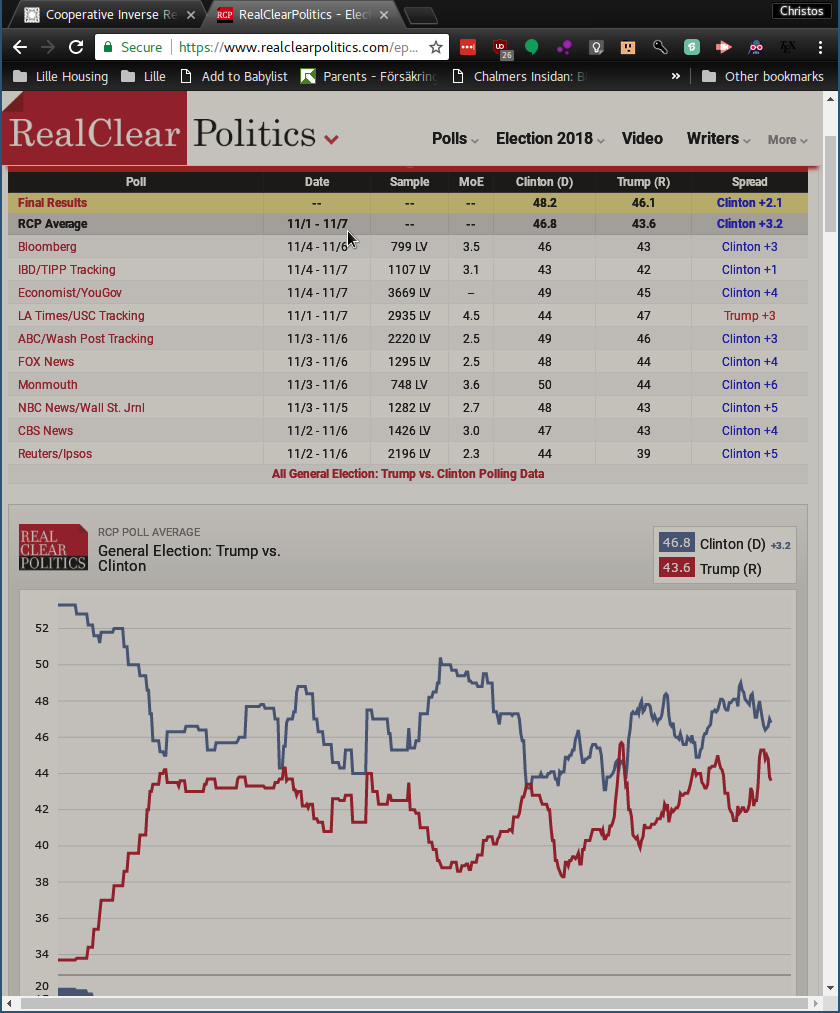
\includegraphics[width=\textwidth]{../figures/2016-election}}
  \only<article>{A simple example is the 2016 election. While we can make models}
  
\end{frame}
\begin{frame}
  \only<article>{The same thing can be done in when dealing purely
    with data, by making sure we use some of the data as input to the
    algorithm, and other data to measure the quality of the algorithm
    itself. In the following, we assume we have some algorithm
    $\alg : \Datasets \to \Pol$, where $\Datasets$ is the universe of
    possible input data and $\Pol$ the possible outputs, e.g. all
    possible classification policies. We also assume the existence of
    some quality measure $U$. How should we measure the quality of our
    algorithmic choices? 
    
    Take classification as an example. For a given training set, simply memorising all the labels of each example gives us perfect performance on the training set. Intuitively, this is not a good measure of performance, as we'd probably get poor results on a freshly sampled set. We can think of the training data as input to an algorithm, and the resulting classifier as the algorithm output. The evaluation function also requires some data in order to measure the performance of the policy. This can be expressed into the following principle.
  }
  \begin{alertblock}{The principle of independent evaluation}    
    Data used for estimation cannot be used for evaluation.
  \end{alertblock}
  \only<article>{This applies both to computer-implemented and human-implemented algorithms.}
\end{frame}


\begin{frame}
  \begin{figure}[H]
    \begin{center}
      \begin{tikzpicture}[line width=2pt]
        \node<1->[select,label=above:Data Collection] at (0,2) (experiment) {$\chi$};
        \node<3->[select,label=below:{Algorithm, hyperparameters}] at (0,0) (alg) {$\alg$};
        \node<2->[RV,label=above:Training] at (4,2) (training) {$\Training$};
        \node<5->[RV,label=above:Holdout] at (8,2) (holdout) {$\Holdout$};
        \draw<2->[blue,->] (experiment) -- (training);
        \draw<6->[blue,->] (experiment) to [bend left=45] (holdout);
        \node<4->[RV,label=below:Classifier] at (4,0) (pol) {$\pol$};
        \draw<4->[red,->,dashed] (experiment) -- (pol);
        \draw<4->[red,->] (alg) -- (pol);
        \draw<4->[red,->] (training) -- (pol);
        \node<7->[utility,label=below:Measurement] at (8,0) (util) {$\util$};
        \draw<7->[red,->] (pol) -- (util);
        \draw<7->[red,->] (holdout) -- (util);
      \end{tikzpicture}
    \end{center}
    \caption{The decision process in classification.}
  \end{figure}
  \only<article>{One can think of the decision process in classification as follows. First, we decide to collect some data according to some experimental protocol $\chi$. We also decide to use some algorithm (with associated hyperparameters) $\alg$ together with data $\Training$ we will obtain from our data collection in order to obtain a classification policy $\pol$. Typically, we need to measure the quality of a policy according to how well it classifies on unknown data. This is because our policy has been generated using $\Training$, and so any measurement of its accuracy is going to be biased.}
  \uncover<5->{
    \begin{block}{Classification accuracy}
      \[
      \E_\chi[\util(\pol)] = \sum_{x,y} \underset{\textrm{Data probability}}{\underbrace{\Pr_\chi(x, y)}} \overset{\textrm{Decision probability}}{\overbrace{\pol(a = y \mid x)}}
      \]
      \only<article>{The classification accuracy of policy $\pol$ under $\chi$ is the expected number of times the policy decides $\pol$ chooses the correct class.}
    \end{block}
  }
\end{frame}

\subsection{The human as an algorithm}
\begin{frame}
  \frametitle{The human as an algorithm.}
  \only<article>{The same way with which an algorithm creates a model from some prior assumptions and data, so can a human select an algorithm and associated hyperparamters by executing an algorithm herself. This involves trying different algorithms and hyperparametrs on the same training data $\Training$ and then measuring their performance in the holdout set $\Holdout$.}
  \begin{figure}[H]
  \centering
  \begin{tikzpicture}[line width=2pt]
    \node[select,label=above:Data Collection] at (0,2) (experiment) {$\chi$};
    \node[RV,label=above:Training] at (4,2) (training) {$\Training$};
    \node[RV,label=above:Holdout] at (8,2) (holdout) {$\Holdout$};
     \draw[blue,->] (experiment) -- (training);
    \draw[blue,->] (experiment) to [bend left=45] (holdout);
    \node<2->[select,label=below:{Algorithm, hyperparameters}] at (0,0) (alg) {$\alg_1$};     
    \node<3->[RV,label=below:Classifier] at (4,0) (pol) {$\pol_1$};
    \draw<3->[red,->] (alg) -- (pol);
    \draw<3->[red,->] (training) -- (pol);
    \node<4->[utility,label=below:Measurement] at (8,0) (util) {$\util_1$};
    \draw<4->[red,->] (pol) -- (util);
    \draw<4->[red,->] (holdout) -- (util);
    \node<5->[select,label=below:{Algorithm, hyperparameters}] at (0,-2) (alg2) {$\alg_2$};
    \node<6->[RV,label=below:Classifier] at (4,-2) (pol2) {$\pol_2$};
    \node<7->[utility,label=below:Measurement] at (8,-2) (util2) {$\util_2$};
    \draw<6->[red,->] (alg2) -- (pol2);
    \draw<6->[red,->] (training) to [bend left] (pol2);
    \draw<7->[red,->] (pol2) -- (util2);
    \draw<7->[red,->] (holdout) to [bend right] (util2);
  \end{tikzpicture}
    \caption{Selecting algorithms and hyperparameters through holdouts}
    \label{fig:human-as-algorithm}
  \end{figure}

\end{frame}

\begin{frame}
  \frametitle{Holdout sets}
  \only<article>{To summarise, holdout sets are used in order to be able to evaluate the performance of specific algorithms, or hyparameter selection.}
  \begin{itemize}
  \item Original data $\Data$, e.g. $\Data = (x_1, \ldots, x_T)$.
  \item Training data $\Training \subset \Data$, e.g. $\Training = x_1, \ldots, x_n$, $n < T$.
  \item Holdout data $\Holdout = D \setminus \Training$, used to measure the quality of the result.
  \item Algorithm $\alg$ with hyperparametrs $\hyperparam$.
  \item Get algorithm output $\pol = \alg(\Training, \hyperparam)$.
  \item Calculate quality of output $U(\pol, \Holdout)$
  \end{itemize}
  \only<article>{
    We start with some original data $\Data$, e.g. $\Data = (x_1, \ldots, x_T)$. We then split this into a training data set $\Training \subset \Data$, e.g. $\Training = x_1, \ldots, x_n$, $n < T$ and holdout dataset $\Holdout = D \setminus \Training$. This is used to measure the quality of selected algorithms $\alg$ and hyperparameters $\hyperparam$. We run an algorithm/hyperparameter combination on the training data and obtain a result $\pol = \alg(\Training, \hyperparam)$.    \footnote{As typically algorithms are maximising the quality metric on the training data, 
    \[
    \alg(\Training) = \argmax_y U(y, \Training)
    \]
    we typically obtain a biased estimate, which depends both on the algorithm itself and the training data. For \KNN{} in particular, when we measure accuracy on the training data, we can nearly always obtain near-perfect accuracy, but not always perfect. Can you explain why?}
 We then calculate the quality of the output $U(\pol, \Holdout)$ on the holdout set.
    Unfortunately, the combination that appears the best due to the holdout result may look inferior in a fresh sample. Following the principle of ``data used for evaluation cannot be used for estimation'', we must measure performance on another sample.
  }
  \begin{block}{Holdout and test sets for unbiased algorithm comparison}
    \only<article>{
      Consider the problem of comparing a number of different algorithms in $\Alg$. Each algorithm $\alg$ has a different set of hyperparameters $\Hyperparam_\alg$. The problem is to choose the best parameters for each algorithm, and then to test them independently. A simple meta-algorithm for doing this is based on the use of a \emph{holdout} set for choosing hyperparameters for each algorithm, and a \emph{test} set to measure algorithmic performance.}
    \begin{algorithm}[H]
      \begin{algorithmic}
        \State Partition data into $\Training, \Holdout, \Testing$.
        \For {$\alg \in \Alg$} \For
        {$\hyperparam \in \Hyperparam_\alg$} \State
        $\pol_{\hyperparam, \alg} = \alg(\Training, \hyperparam)$.
        \EndFor
        \State Get $\pol^*_{\alg}$ maximising
        $\util(\pol_{\hyperparam, \alg}, \Holdout)$.  \State
        $u_\alg = \util(\pol^*_\alg, \Testing)$.
        \EndFor
        \State $\alg^* = \argmax_\alg u_\alg$.
      \end{algorithmic}
      \caption{Unbiased adaptive evaluation through data partitioning}
    \end{algorithm}
  \end{block}
  \only<article>{This ensures that we are not biased in our decision about what is the best algorithm.}
\end{frame}

\begin{frame}
  \frametitle{Final performance measurement}
  \begin{figure}[H]
    
    \centering
  \begin{tikzpicture}[line width=2pt]
    \node[select,label=above:Data Collection] at (0,0) (experiment) {$\chi$};
    \node[RV,label=above:Training] at (2,0) (training) {$\Training$};
    \node[RV,label=above:Holdout] at (4,0) (holdout) {$\Holdout$};
    \node[RV,label=above:Testing] at (6,0) (testing) {$\Testing$};
    \draw[blue,->] (experiment) -- (training);
    \draw[blue,->] (experiment) to [bend left=15] (holdout);
    \draw[blue,->] (experiment) to [bend left=45] (testing);
    \node[select,label=below:{human}] at (0,-2) (human) {$\eta$};
    \node[RV,label=below:Algorithm 1] at (2,-2) (alg1) {$\alg_1$};
    \node[RV,label=below:Classifier 1] at (4,-2) (pol1) {$\pol_1$};
    \node[RV,label=below:Result 1] at (6,-2) (util1) {$\util^*_1$};
    \node[RV,label=below:Algorithm 2] at (2,-4) (alg2) {$\alg_2$};
    \node[RV,label=below:Classifier 2] at (4,-4) (pol2) {$\pol_2$};
    \node[RV,label=below:Result 2] at (6,-4) (util2) {$\util^*_2$};
    \draw[->,red] (human) -- (alg1);
    \draw[->,red] (alg1) -- (pol1);
    \draw[->,red] (pol1) -- (util1);
    \draw[->,red] (human) -- (alg2);
    \draw[->,red] (alg2) -- (pol2);
    \draw[->,red] (pol2) -- (util2);
    \draw[->,red] (training) -- (pol1);
    \draw[->,red] (holdout) -- (pol1);
    \draw[->,red] (testing) -- (util1);
    \draw[->,red] (training) -- (pol2);
    \draw[->,red] (holdout) to [bend left = 45] (pol2);
    \draw[->,red] (testing) to [bend left = 45] (util2);
  \end{tikzpicture}
  \only<article>{
    \caption{Simplified dependency graph for selecting hyperparameters for different algorithms, and comparing them on an independent test set. For the $i$-th algorithm, the classifier model is }
  }
\end{figure}
\end{frame}

\subsection{Algorithmic sensitivity}
\only<article>{The algorithm's output does have a dependence on its input, obviously. So, how sensitive is the algorithm to the input?}
\begin{frame}
  \frametitle{Independent data sets}
  \only<article>{One simple idea is to just collect independent datasets and see how the output of the algorithm changes when the data changes. However, this is quite expensive, as it not might be easy to collect data in the first place.}
  \centering
  \begin{tikzpicture}[line width=2pt]
    \node[select,label=above:Experiment] at (0,0) (experiment) {$\chi$};
    \node[select,label=below:{Algorithm}] at (8,0) (alg) {$\alg$};
    \node[RV,label=below:1st sample] at (4,0) (sample1) {$D_1$};
    \node[RV,label=below:1st Result] at (6,0) (pol1) {$\pol_1$};
    \node<2>[RV,label=above:2nd Sample] at (4,2) (sample2) {$D_2$};
    \node<2>[RV,label=above:2nd Result] at (6,2) (pol2) {$\pol_2$};
        \draw[blue,->] (experiment) -- (sample1);
    \draw[red,->] (alg) -- (pol1);
    \draw[red,->] (sample1) -- (pol1);
    \draw<2>[blue,->] (experiment) -- (sample2);
    \draw<2>[red,->] (alg) -- (pol2);
    \draw<2>[red,->] (sample2) -- (pol2);
  \end{tikzpicture}
\end{frame}
\begin{frame}
  \frametitle{Bootstrap samples}
  \only<article>{A more efficient idea is to only collect one dataset, but then use it to generate more datasets. The simplest way to do that is by sampling with replacement from the original dataset, new datasets of the same size as the original. Then the original dataset is sufficiently large, this is approximately the same as sampling independent datasets.}
  \centering
  \begin{tikzpicture}[line width=2pt]
    \node[select,label=above:Experiment] at (0,0) (experiment) {$\chi$};
    \node[RV,label=below:training] at (2,0) (training) {$\Training$};
    \draw[blue,->] (experiment) -- (training);
    \node[select,label=below:{Algorithm}] at (8,0) (alg) {$\alg$};
    \node[RV,label=below:1st sample] at (4,0) (sample1) {$D_1$};
    \node[RV,label=below:1st Result] at (6,0) (pol1) {$\pol_1$};
    \node[RV,label=above:2nd Sample] at (4,2) (sample2) {$D_2$};
    \node[RV,label=above:2nd Result] at (6,2) (pol2) {$\pol_2$};
    \draw[red,->] (alg) -- (pol1);
    \draw[red,->] (sample1) -- (pol1);
    \draw[red,->] (training) -- (sample1);
    \draw[red,->] (training) -- (sample2);
    \draw[red,->] (alg) -- (pol2);
    \draw[red,->] (sample2) -- (pol2);
  \end{tikzpicture}
  \only<article>{As usual, we can evaluate our algorithm on an independent holdout set.}
\end{frame}



\begin{frame}
  \frametitle{Bootstrapping}
  Bootstrapping is a general technique that can be used to:
  \begin{itemize}
  \item Estimate the sensitivity of $\alg$ to the data $x$.
  \item Obtain a distribution of estimates $\pol$ from $\alg$ and the data $x$.
  \end{itemize}
  \begin{block}{Bootstrapping}
    \begin{enumerate}
    \item \textbf{Input} Training data $\Data$, number of samples $k$.
    \item \textbf{For} $i = 1, \ldots, k$
    \item \quad $\Data^{(i)} = \textrm{Bootstrap}(\Data)$
    \item \textbf{return} $\cset{\Data^{(i)}}{i = 1, \ldots, k}$.
    \end{enumerate}
    where  $\textrm{Bootstrap}(\Data)$ samples with replacement $|\Data|$ points from $\Training$.
  \end{block}
\end{frame}


\begin{frame}
\frametitle{Cross-validation}
  \begin{block}{$k$-fold Cross-Validation}
    \begin{enumerate}
    \item \textbf{Input} Training data $\Training$, number of folds $k$, algorithm $\alg$, measurement function $\util$
    \item Create the partition $\Data^{(1)} \ldots, \Data^{(k)}$ so that $\bigcup_{i=1}^k \Data^{(k)} = \Data$.
    \item Define $\Training^{(i)} = \Data \setminus \Data^{(i)}$
    \item \quad $\pol_i = \alg(\Training^{(i)})$
    \item \textbf{For} $i = 1, \ldots, k$:
    \item \quad $\pol_i = \alg(\Data^{(i)})$
    \item \quad $u_i = \util(\pol_i)$
    \item \textbf{return} $\{y_1, \ldots, y_i\}$.
    \end{enumerate}
  \end{block}
\end{frame}
\begin{frame}
\frametitle{Independent replication}
\only<article>{The gold standard for reproducibility is independent replication. Simply have another team try and reproduce the results you obtained, using completely new data. If the replication is successful, then you can be pretty sure there was no flaw in your original analysis.}
\begin{block}{Replication study}
  \begin{enumerate}
  \item Reinterpret the original hypothesis and experiment.
  \item Collect data according to the original protocol, \alert{unless flawed}. \only<article>{It is possible that the original experimental protocol had flaws. Then the new study should try and address this through an improved data collection process. For example, the original study might not have been double-blind. The new study can replicate the results in a double-blind regime.}
  \item Run the analysis again, \alert{unless flawed}. \only<article>{It is possible that the original analysis had flaws. For example, possible correlations may not have been taken into account.}
  \item See if the conclusions are in agreement.
  \end{enumerate}
\end{block}
\end{frame}



%%% Local Variables:
%%% mode: latex
%%% TeX-master: "notes"
%%% End:

